\section{Scheduler}

Depuis sa version 2.6.23 le kernel utilise le Completely Fair Scheduler (CFS),
il est aujourd'hui le scheduler par défaut. Le but du CFS est de proposer un ordonnancement
idéal pour le multitasking, où la puissance du CPU est partagée entre les processus.
Or ce modèle n'est pas possible, un CPU ne peut exécuter qu'un flot d'exécution à la
fois. Dans cette partie nous introduirons les mécanismes mis en œuvre par le CFS pour
imiter un multitasking parfait. 

\subsection{L'arbre rbtree}
Le CFS fonctionne sur un système d'arbre: le \verb|rbtree|. L'arbre permet de
créer une timeline sur les futures tâches à exécuter.
Il est composé de \verb|sched_entity|, ces entités regroupent une ou plusieurs
tâches, permettant ainsi de faire des lots d'exécution. Chaque entité a un compteur
du temps d'exécution virtuel passé dans le
CPU nommé \verb|vruntime|. Cela permet au scheduler d'organiser son
arbre d'exécution: les entités sont réparties par ordre croissant à partir de
leur \verb|vruntime|, de gauche à droite. Ainsi, à gauche de l'arbre se trouve
l'entité avec la valeur \verb|vruntime| la plus faible, c'est cette entité qui
sera choisie lors de l'élection par le scheduler.

\subsection{Poids et timeslice}
L'équité est le maître mot du scheduler CFS. Chaque tâche se voit attribuer un poids
(\verb|load|) calculé dépendamment des autres tâches exécutables et de leur priorité.
Le CFS introduit un \verb|target time|, cette valeur correspond aux temps CPU que doit se partager
les tâches exécutables en fonction de leur poids. Le temps d'exécution attribué sur le CPU pour 
chaque tâche est nommé \verb|timeslice| et est calculé à partir de son poids et 
du \verb|target time|. Ainsi, une tâche avec une priorité plus élevée aura un poids 
plus important et donc un \verb|timeslice| plus grand.
Prenons un exemple, deux tâches de  même priorité doivent se partager un 
\verb|target time| de 10 ms. Les deux tâches ont donc le même poids, le CFS attribuera 
aux tâches un \verb|timeslice| de 5 ms. Si nous prenons 
maintenant deux tâches où leur différence de priorité est de 5, soit par 
exemple 10 et 15, avec un \verb|target time| de 20 ms, le poids diffère et la 
tâche la moins prioritaire se verra attribuer 1/3 du \verb|target time| soit 
une \verb|timeslice| de 5 ms contre 15 ms pour l'autre tâche.

\subsection{Horloge virtuelle}
Le cœur du fonctionnement du CFS se repose sur son horloge virtuelle : la
\verb|virtual clock|. Cette horloge permet au scheduler de mesurer un temps
d'exécution virtuel sur le CPU pour chaque entité. Cette valeur est stockée dans
la variable \verb|vruntime|. L'entité élue se voit mettre à jour ses statistiques
fréquemment, c'est ici que sa valeur \verb|vruntime| est mise à jour. Le
principe est le suivant : à chaque fois qu'une entité s'exécute dans le CPU le
timestamp est sauvegardé dans la variable \verb|exec_start|, à chaque mise à
jour de \verb|vruntime| la différence entre le timestamp actuelle et
\verb|exec_start| est calculée dans la variable \verb|delta_exec|, la valeur de
cette dernière sera divisé par le poids de l'entité puis ajouté au
\verb|vruntime|. Ainsi, plus la priorité est élevée plus la valeur ajoutée au
\verb|vruntime| sera faible et par conséquent l'entité avancera lentement vers
la droite de l'arbre (Figure \ref{fig:sched}).
\begin{figure}[h!]
	\centering
	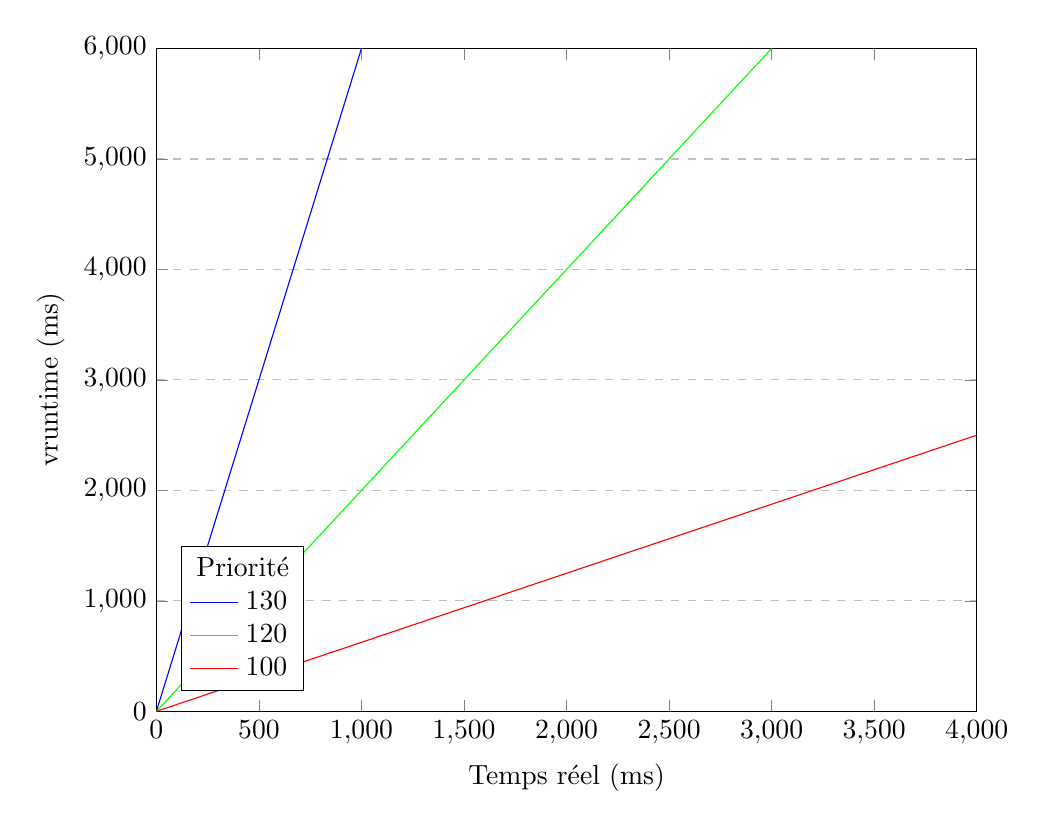
\begin{tikzpicture}
	\begin{axis}[
	xlabel={Temps réel (ms)},
	ylabel={vruntime (ms)},
	xmin=0, xmax=4000,
	ymin=0, ymax=6000,
	legend pos=south west,
	ymajorgrids=true,
	grid style=dashed,
	width=12cm,height=10cm,
	]
	
	\addlegendimage{empty legend}
	
	\addplot[
	color=blue,
	]
	coordinates {
		(0,0)(1000,6000)
	};
	
	\addplot[
	color=green,
	]
	coordinates {
		(0,0)(3000,6000)
	};
	
	\addplot[
	color=red,
	]
	coordinates {
		(0,0)(4000,2500)
	};
	\addlegendentry{\hspace{-.6cm}Priorité}
	\addlegendentry{130}
	\addlegendentry{120}
	\addlegendentry{100}
	
	\end{axis}
	\end{tikzpicture}
	\caption{Relation entre le vruntime et le temps réel en fonction de la priorité}
	\label{fig:sched}
\end{figure}


Pour prioriser une entité nous pouvons influencer son 
\verb|vruntime| pour la garder à gauche de l'arbre et assurer une réélection 
rapide. Étant donné que la valeur \verb|vruntime| se base sur la priorité de 
l'entité nous avons décidé d'influencer la priorité des processus, et 
les utiliser comme un levier pour dire au scheduler de favoriser l'élection 
du processus qui détient le verrou. Pour cause, la modification du scheduler aurait
demandé d'étudier et de maîtriser tout le code et les détails du scheduler, afin
d'être sûr que nos modifications ne compromettent pas son fonctionnement.